\documentclass[preprint,12pt,authoryear]{elsarticle}

\usepackage{hyperref}
\usepackage{natbib}
\usepackage{graphicx}
\usepackage{ifthen}
\usepackage{tabularx}
\usepackage{lineno}
\linenumbers*[1]

% add references to research questions in margin
\newcommand{\mrq}[2][]{}
\newcommand{\rrq}[3][]{}
\newboolean{ispaper}
\setboolean{ispaper}{true}

\def\appendixname{}

\journal{Coastal Engineering}

\begin{document}

\begin{figure}
  \centering
  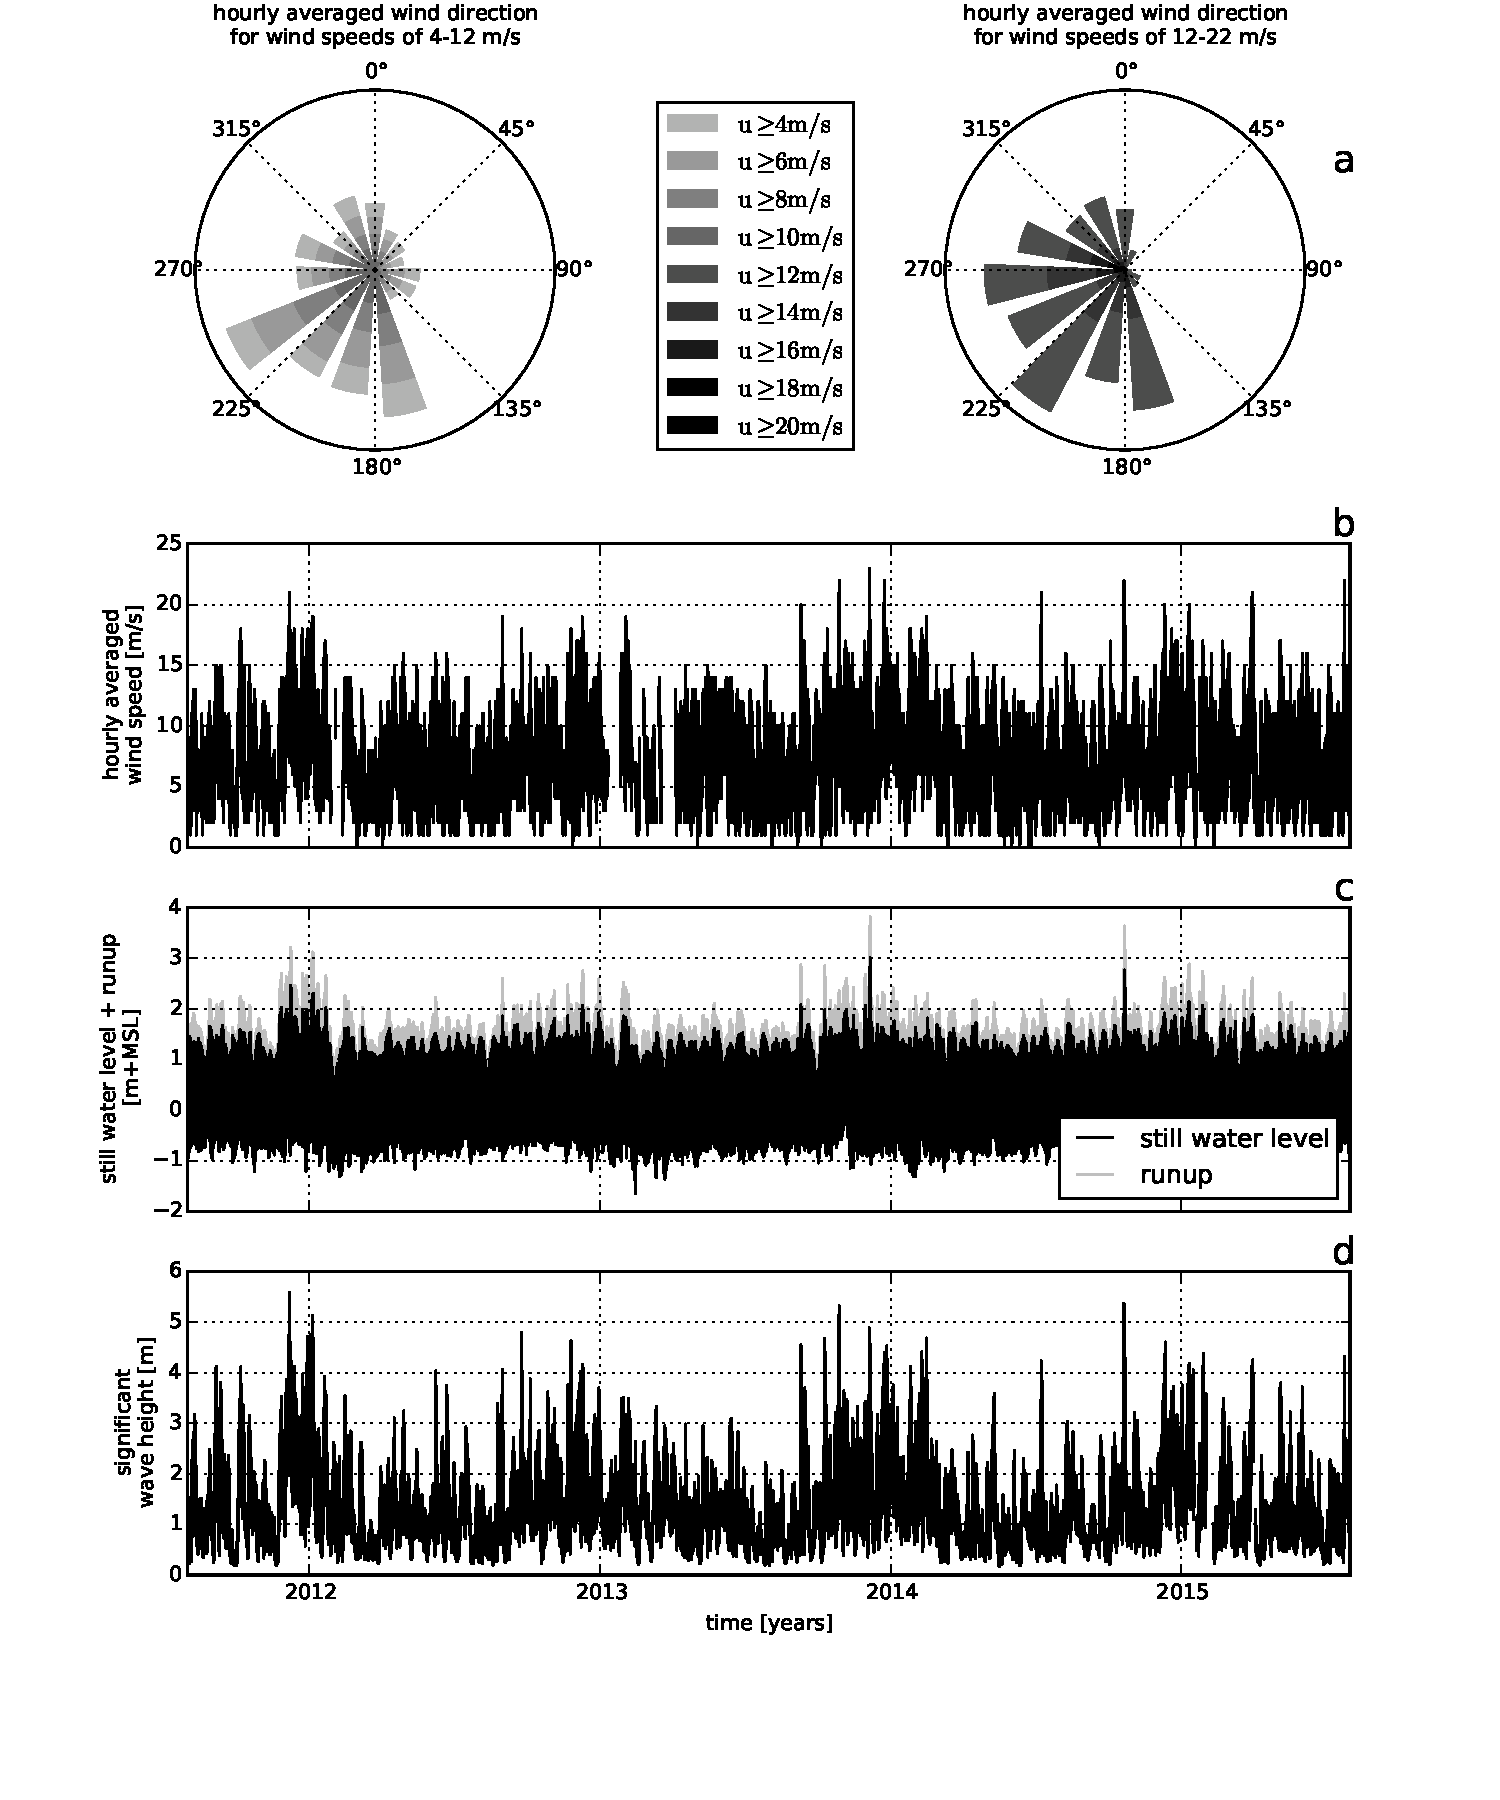
\includegraphics[width=\columnwidth]{../Figures/boundaryconditions}
  \caption{Wind and hydrodynamic time series from 2011 to 2015. Hourly
    averaged wind speeds and directions are obtained from the KNMI
    meteorological station in Hoek van Holland (upper
    panels). Offshore still water levels, wave heights and wave
    periods are obtained from the Europlatform (lower panels). Runup
    levels are estimated following \citet{Stockdon2006}.}
  \label{fig:windwaves}
\end{figure}

\appendix

\ifthenelse{\boolean{ispaper}}{
  \section{Theoretical Sediment Transport Volumes}
}{
  \chapter{Theoretical Sediment Transport Volumes}
}\label{apx:theoretical_transport}

The cumulative theoretical sediment transport volume $Q$
[$\mathrm{m^3}$] in the Sand Motor domain between September 1, 2011
and September 1, 2015 is estimated from hourly averaged measured wind
speed $u_{10}$ [m/s] and direction $\theta_u$ [$^{\circ}$] measured at
10 m height by the KNMI meteorological station in Hoek van Holland
(Figure \ref{fig:windwaves}). The wind time series are used in
conjunction with the formulation of \citet{Bagnold1937a} to obtain the
instantaneous theoretical sediment transport rate $q$ [kg/m/s]
following:

\begin{equation}
  q = C \frac{\rho_{\mathrm{a}}}{g} \sqrt{\frac{d_{\mathrm{n}}}{D_{\mathrm{n}}}} \left(u_{\mathrm{*}} - u_{\mathrm{* th}} \right)^3
\end{equation}

\noindent with the shear velocity
$u_{\mathrm{*}} = \alpha \cdot u_{10}$ m/s, the shear velocity
threshold $u_{\mathrm{* th}} = \alpha \cdot 3.87$ m/s, the conversion
factor from free-flow wind velocity to shear velocity
$\alpha = 0.058$, the air density $\rho_{\mathrm{a}}$ = 1.25
$\mathrm{kg/m^3}$, the particle density $\rho_{\mathrm{p}}$ = 2650.0
$\mathrm{kg/m^3}$, the gravitational constant $g$ = 9.81
$\mathrm{m/s^2}$, the nominal grain size $d_{\mathrm{n}}$ = 335
$\mu \mathrm{m}$ and a reference grain size $D_{\mathrm{n}}$ = 250
$\mu \mathrm{m}$.

The cumulative theoretical sediment transport volumes in onshore
($Q_{\mathrm{os}}$ [$\mathrm{m^3}$]) and alongshore ($Q_{\mathrm{as}}$
[$\mathrm{m^3}$]) direction are computed by time integration and
conversion from mass to volume following:

\begin{equation}
  \label{eq:apx_theoretical_transport}
  \begin{array}{lclcl}
    Q_{\mathrm{os}} &=& \sum q \cdot \frac{\Delta t \cdot \Delta y}{(1 - p) \cdot \rho_{\mathrm{p}}} \cdot f_{\theta_u,\mathrm{os}} &=& 110 \cdot 10^4 ~ \mathrm{m^3} \\
    Q_{\mathrm{as}} &=& \sum q \cdot \frac{\Delta t \cdot \Delta x}{(1 - p) \cdot \rho_{\mathrm{p}}} \cdot f_{\theta_u,\mathrm{as}} &=& 3 \cdot 10^4 ~ \mathrm{m^3} \\
  \end{array}
\end{equation}

\noindent where the temporal resolution $\Delta t$ = 1 h, the
alongshore span of the measurement domain $\Delta y$ = 4 km, the
approximate lateral beach width $\Delta x$ = 100 m, the porosity $p$ =
0.4 and $f_{\theta_u,\mathrm{os}}$ and $f_{\theta_u,\mathrm{as}}$ are
factors to account for respectively the onshore and alongshore wind
directions only, defined as:

\begin{equation}
  \begin{array}{lcl}
    f_{\theta_u,\mathrm{os}} &=& \max \left( 0 \quad ; \quad \cos \left( 312\,^{\circ} - \theta_u \right) \right) \\
    f_{\theta_u,\mathrm{as}} &=& \sin \left( 312\,^{\circ} - \theta_u \right) \\
  \end{array}
\end{equation}

\noindent where $\theta_u$ [$^{\circ}$] is the hourly averaged wind
direction and $312\,^{\circ}$ accounts for orientation of the original
coastline.

Note that the difference between the onshore and alongshore cumulative
theoretical sediment transport volumes (Equation
\ref{eq:apx_theoretical_transport}) of a factor 40 is determined
solely by the difference between the onshore and alongshore
cross-sections of 4 km and 100 m respectively. The sediment transport
volumes per meter width in onshore and alongshore direction are of the
same order of magnitude (275 $\mathrm{m^3/m}$ and 267 $\mathrm{m^3/m}$
respectively).

%%% Local Variables:
%%% mode: latex
%%% TeX-master: "./thesis"
%%% End:


\section*{References}
\bibliographystyle{apalike} %elsarticle-harv}
\bibliography{bibliography}{}

\end{document}

%%% Local Variables:
%%% mode: latex
%%% TeX-master: t
%%% End:
